\changecolours{ScoutGreen}
\section{Arquitetura em Memória e Mecanismos de Persistência}

% ------------------------------------------------------------------------------
\twocolframe[title={A Memória RAM: Velocidade Extrema vs Volatilidade},leftcol=7cm,rightcol=7cm]{%
  \alert{Por que o Redis é Tão Rápido?}\par
  \itemseps[topsepi=2mm,itemsepi=3mm,labelsep=2mm,leftmargini=4mm]
  \begin{itemize}
    \item Acesso direto à memória RAM sem overhead de barramento mecânico ou NVMe.
    \item Latência típica: \textbf{70 microssegundos} ($\approx 0,07$ ms).
    \item \textbf{O Dilema Físico:} A memória RAM é \textbf{volátil}. Se o servidor reiniciar ou faltar energia, todos os dados são apagados.
  \end{itemize}
}{%
  \alert{A Solução: Persistência em Disco}\par
  \itemseps[topsepi=2mm,itemsepi=3mm,labelsep=2mm,leftmargini=4mm]
  \begin{itemize}
    \item O Redis não é apenas um cache efêmero; ele pode operar como banco de dados durável.
    \item O motor oferece dois mecanismos nativos de armazenamento não-volátil:
    \item \textbf{1. RDB (Snapshotting):} Fotografias pontuais em disco.
    \item \textbf{2. AOF (Append-Only File):} Diário contínuo de operações.
  \end{itemize}
}

% ------------------------------------------------------------------------------
\begin{frame}{Arquitetura em Memória vs Armazenamento Persistente}
  \centering
  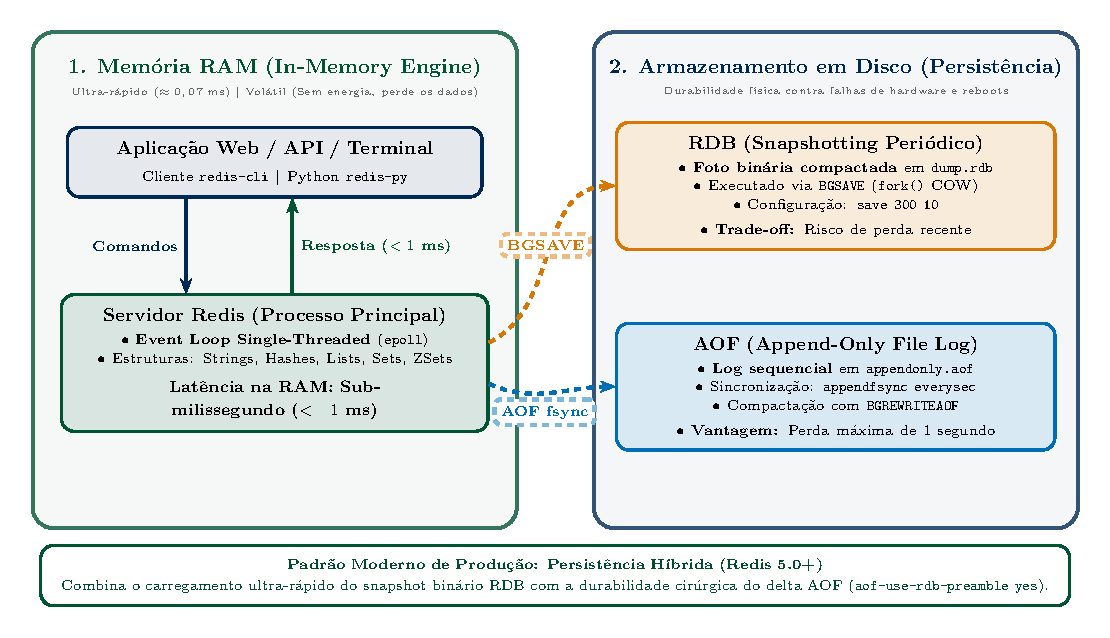
\includegraphics[width=0.90\textwidth,height=0.74\textheight,keepaspectratio]{figuras/fig_arquitetura_memoria_persistencia.pdf}
\end{frame}

% ------------------------------------------------------------------------------
\twocolframe[title={Mecanismo 1: RDB (Snapshotting e BGSAVE)},leftcol=7cm,rightcol=7cm]{%
  \alert{Como Funciona o Snapshotting}\par
  \itemseps[topsepi=2mm,itemsepi=3mm,labelsep=2mm,leftmargini=4mm]
  \begin{itemize}
    \item O RDB grava uma cópia binária compactada de toda a memória no arquivo \texttt{dump.rdb}.
    \item Ideal para \textbf{backups periódicos} e recuperação de desastres.
    \item \textbf{Ponto de Restauração:} Se houver falha, dados gerados após o último snapshot são perdidos.
  \end{itemize}
}{%
  \alert{Diferença Crítica: BGSAVE vs SAVE}\par
  \itemseps[topsepi=2mm,itemsepi=3mm,labelsep=2mm,leftmargini=4mm]
  \begin{itemize}
    \item \textbf{SAVE (Síncrono / Bloqueante):} Trava a thread do Redis. Nenhuma consulta é respondida até terminar. \textbf{Nunca use em produção!}
    \item \textbf{BGSAVE (Assíncrono / Não-bloqueante):} Dispara processo filho via \texttt{fork()} com \textit{Copy-on-Write} (COW). Atende conexões sem interrupção.
  \end{itemize}
}

% ------------------------------------------------------------------------------
\begin{frame}[fragile]{Configuração do RDB e Comandos no redis-cli}
  \begin{columns}[T]
    \begin{column}{0.48\textwidth}
      \alert{Regras de Disparo no redis.conf}\par
      \begin{lstlisting}[language=bash]
# Sintaxe: save <segundos> <alteracoes>
save 900 1      # 15 min se 1 chave mudou
save 300 10     # 5 min se 10 chaves mudaram
save 60 10000   # 1 min se 10k chaves mudaram

# Destino do snapshot binario
dbfilename dump.rdb
dir /var/lib/redis
      \end{lstlisting}
    \end{column}
    \begin{column}{0.50\textwidth}
      \alert{Disparo Manual via redis-cli}\par
      \begin{lstlisting}[language=bash]
# Disparar snapshot assincrono:
127.0.0.1:6379> BGSAVE
Background saving started

# Timestamp UNIX do ultimo dump:
127.0.0.1:6379> LASTSAVE
(integer) 1791888929

# Inspecionar status de persistencia:
127.0.0.1:6379> INFO persistence
# rdb_last_bgsave_status:ok
      \end{lstlisting}
    \end{column}
  \end{columns}
\end{frame}

% ------------------------------------------------------------------------------
\twocolframe[title={Mecanismo 2: AOF (Append-Only File)},leftcol=7cm,rightcol=7cm]{%
  \alert{Diário Sequencial de Operações}\par
  \itemseps[topsepi=2mm,itemsepi=3mm,labelsep=2mm,leftmargini=4mm]
  \begin{itemize}
    \item Registra cada comando de escrita recebido em modo append (\texttt{appendonly.aof}).
    \item Na reinicialização, o Redis reproduz o diário para reconstruir o estado com quase zero perda.
    \item \textbf{BGREWRITEAOF:} Compacta o diário em background removendo comandos obsoletos.
  \end{itemize}
}{%
  \alert{Políticas de Sincronização (fsync)}\par
  \itemseps[topsepi=2mm,itemsepi=3mm,labelsep=2mm,leftmargini=4mm]
  \begin{itemize}
    \item \textbf{appendfsync always:} Sincroniza a cada comando. Durabilidade máxima, menor vazão.
    \item \textbf{appendfsync everysec (Padrão Recomendado):} Descarrega em disco a cada 1 segundo. Máxima perda: 1 segundo de dados.
    \item \textbf{appendfsync no:} O SO decide quando gravar.
  \end{itemize}
}

% ------------------------------------------------------------------------------
\begin{frame}[fragile]{Configuração do AOF e Persistência Híbrida}
  \begin{columns}[T]
    \begin{column}{0.48\textwidth}
      \alert{Diretivas no redis.conf}\par
      \begin{lstlisting}[language=bash]
# Habilitar o modo Append-Only
appendonly yes
appendfilename "appendonly.aof"

# Frequencia de flush fsync em disco
appendfsync everysec

# Persistencia Hibrida (Padrao Redis 5+)
# Salva RDB no inicio + AOF no final
aof-use-rdb-preamble yes
      \end{lstlisting}
    \end{column}
    \begin{column}{0.50\textwidth}
      \alert{Compactação e Inspecção no CLI}\par
      \begin{lstlisting}[language=bash]
# Reescrever diario AOF em background:
127.0.0.1:6379> BGREWRITEAOF
Background append only file rewriting started

# Consultar estatisticas detalhadas:
127.0.0.1:6379> INFO persistence
# aof_enabled:1
# aof_rewrite_in_progress:0
      \end{lstlisting}
    \end{column}
  \end{columns}
\end{frame}
